%----------------------------------------------------------------------------------------
% RADIALEN EN DE EENHEIDSCIRKEL. Alle opgaven zijn eigen werk.
%
% Opbouw: Start, leerstof (theorie, werkwijze of uitleg, voorbeeld, korte oefening), en op een
% nieuwe pagina de Opdrachten (door elkaar, stijgende moeilijkheid), Koppel en Test jezelf.
% Labels van dit hoofdstuk beginnen met h1-.
%----------------------------------------------------------------------------------------

\mychapter{1}{De eenheidscirkel}

\lkr{Leerplan B+S: LPD 13-16 (goniometrische functies), het deel over radialen, georiënteerde hoeken en de goniometrische getallen op de goniometrische cirkel. Uit de 2de graad kennen leerlingen sinus, cosinus en tangens in een rechthoekige driehoek, in graden. Laat de bijzondere waarden niet van buiten leren zonder figuur: de twee tekendriehoeken en de eenheidscirkel volstaan om ze altijd terug te vinden.}

In de 2de graad waren sinus, cosinus en tangens verhoudingen van zijden in een rechthoekige driehoek, voor hoeken tussen $0^\circ$ en $90^\circ$. Een rad, een golf of een slinger draait echter verder dan $90^\circ$, en soms in tegenwijzerzin. Daarom breiden we de goniometrische getallen uit tot \textit{alle} hoeken, met de eenheidscirkel. En we meten hoeken voortaan in radialen.

Dit hoofdstuk legt de basis voor de rest van de cursus: de formules van hoofdstuk 2, de grafieken van hoofdstuk 3 en de vergelijkingen van hoofdstuk 4 vertrekken allemaal van het punt dat over de eenheidscirkel draait.

\begin{oefeningen}[Start]
\oef{h1-start-1}

\oef{h1-verken}
\end{oefeningen}

%========================================================================================
\section{Radialen}

Dat een volle toer $360^\circ$ is, is een afspraak die al uit de oudheid stamt. Het getal $360$ heeft niets met de cirkel zelf te maken. Een natuurlijkere maat vertrekt van de cirkel: hoeveel keer past de straal op de boog die de hoek afsnijdt?

\subsection{De radiaal}

\naast{%
\begin{theorie}
Een hoek van \textbf{\textcolor{accent}{1 radiaal}} (1 rad) is de middelpuntshoek die op een cirkel met straal $r$ een boog met lengte $r$ afsnijdt.
\end{theorie}
Op de figuur rechts is de gekleurde boog even lang als de straal. Die hoek is ongeveer $57^\circ$: iets kleiner dan de hoek van $60^\circ$ in een gelijkzijdige driehoek, want de boog is langer dan de rechte zijde.}{%
\begin{tikzpicture}[scale=1.25,font=\scriptsize]
  \fill[accent!15] (0,0) -- (0:1) arc (0:57.3:1) -- cycle;
  \draw[grijs] (0,0) circle (1);
  \draw[accent,thick] (0:1) arc (0:57.3:1);
  \draw (0,0) -- node[below] {$r$} (1,0);
  \draw (0,0) -- node[above left] {$r$} (57.3:1);
  \node[accent] at (28:1.2) {$r$};
  \node at (25:.4) {$1$ rad};
\end{tikzpicture}}

Hoeveel radialen is een volle toer? Dat hangt niet af van de straal: op een grote cirkel is de boog langer, maar de straal ook.

\begin{theorie}
\begin{stelling}{Graden en radialen}
\qquad $\formule{180^\circ = \pi \text{ rad}}$
\end{stelling}
\begin{bewijs}
Een boog is evenredig met zijn middelpuntshoek. Een volle hoek snijdt de hele omtrek $2\pi r$ af, en die is $2\pi$ keer zo lang als de boog $r$ bij een hoek van $1$ rad. Een volle hoek is dus $2\pi$ rad:
\bewijsregel{360^\circ = 2\pi \text{ rad}, \quad \text{zodat} \quad 180^\circ = \pi \text{ rad}.}
\end{bewijs}
\end{theorie}

Delen door $\pi$ geeft $1 \text{ rad} = \frac{180^\circ}{\pi} \approx 57{,}3^\circ$, en delen door $180$ geeft $1^\circ = \frac{\pi}{180}$ rad. De hoeken die je het vaakst tegenkomt, zijn breuken met $\pi$:

\figuren{\renewcommand{\arraystretch}{1.6}%
\begin{tabular}{|c|*{9}{>{\centering\arraybackslash}p{.95cm}|}}
\hline
graden & $0^\circ$ & $30^\circ$ & $45^\circ$ & $60^\circ$ & $90^\circ$ & $120^\circ$ & $180^\circ$ & $270^\circ$ & $360^\circ$ \\ \hline
radialen & $0$ & $\tfrac{\pi}{6}$ & $\tfrac{\pi}{4}$ & $\tfrac{\pi}{3}$ & $\tfrac{\pi}{2}$ & $\tfrac{2\pi}{3}$ & $\pi$ & $\tfrac{3\pi}{2}$ & $2\pi$ \\ \hline
\end{tabular}}

Vanaf nu meten we hoeken in radialen, tenzij er een gradenteken staat. Het woord rad laten we meestal weg: $\sin 2$ is de sinus van een hoek van $2$ rad.

\voorbeeld{}{Zet $135^\circ$ om naar radialen.\label{vb:h1-radialen}}{%
\uitleg{Een graad is $\frac{\pi}{180}$ rad. We vermenigvuldigen dus met $\frac{\pi}{180}$, en vereenvoudigen de breuk.}
\begin{stappenbreed}
135^\circ = 135 \cdot \frac{\pi}{180} & Elke graad is $\frac{\pi}{180}$ rad. \\[1.5ex]
= \frac{135}{180}\,\pi = \frac{3\pi}{4} & Deel teller en noemer door $45$. Het antwoord is exact, met $\pi$.
\end{stappenbreed}
Controle: $135^\circ = 90^\circ + 45^\circ$, en $\frac{\pi}{2} + \frac{\pi}{4} = \frac{3\pi}{4}$.}

\voorbeeld{}{Zet $2{,}5$ rad om naar graden.\label{vb:h1-graden}}{%
\uitleg{Een radiaal is $\frac{180^\circ}{\pi}$. Hier staat geen $\pi$ in de hoek, dus het antwoord wordt een benadering.}
\begin{stappenbreed}
2{,}5 \text{ rad} = 2{,}5 \cdot \frac{180^\circ}{\pi} & Elke radiaal is $\frac{180^\circ}{\pi}$. \\[1.5ex]
\approx 143{,}2^\circ & Rekentoestel.
\end{stappenbreed}
Controle: $2{,}5$ ligt tussen $\frac{\pi}{2} \approx 1{,}57$ en $\pi \approx 3{,}14$, dus de hoek ligt tussen $90^\circ$ en $180^\circ$.}

\begin{werkwijze}
Van graden naar radialen: vermenigvuldig met $\frac{\pi}{180}$ en vereenvoudig de breuk. Van radialen naar graden: vermenigvuldig met $\frac{180}{\pi}$. Controleer met een hoek uit de tabel die in de buurt ligt.
\end{werkwijze}

\begin{oefeningen}
\oef{h1-radialen}
\end{oefeningen}

\subsection{Booglengte}

Waarom zijn radialen zo handig? Omdat de lengte van een boog dan een eenvoudige formule heeft. In graden is de boog bij een hoek $\alpha$ het deel $\frac{\alpha}{360}$ van de omtrek, met een lastige factor. In radialen valt die factor weg.

\begin{theorie}
\begin{stelling}{Booglengte}
Een middelpuntshoek van $\theta$ rad snijdt op een cirkel met straal $r$ een boog af met lengte

\vspace{1mm}
\qquad $\formule{s = r\theta}$
\end{stelling}
\begin{bewijs}
Een boog is evenredig met zijn middelpuntshoek. Een hoek van $1$ rad snijdt een boog met lengte $r$ af, dus een hoek van $\theta$ rad een boog die $\theta$ keer zo lang is: $s = \theta \cdot r$.
\end{bewijs}
\end{theorie}

Op de eenheidscirkel is $r = 1$, en dan is $s = \theta$: de hoek in radialen \textit{is} de lengte van de boog. Omgekeerd is $\theta = \frac{s}{r}$: een hoek in radialen is een verhouding van twee lengtes, en heeft dus geen eenheid.

\voorbeeld{}{Een pizzapunt heeft straal $15$ cm en een tophoek van $0{,}8$ rad. Hoe lang is de korst?\label{vb:h1-boog}}{%
\uitleg{De korst is de boog van de cirkel, met de tophoek als middelpuntshoek. Die hoek staat al in radialen, dus we passen de formule meteen toe.}
\begin{stappenbreed}
s = r\theta = 15 \cdot 0{,}8 & Straal maal hoek in radialen. \\
= 12 & De korst is $12$ cm lang.
\end{stappenbreed}
Controle: $0{,}8$ rad is iets minder dan $1$ rad, dus de korst is iets korter dan de straal van $15$ cm.}

\begin{oefeningen}
\oef{h1-boog-k}
\end{oefeningen}

\subsection{Sectoroppervlakte}

Ook de oppervlakte van een cirkelsector, een taartpunt, wordt eenvoudig in radialen.

\begin{theorie}
\begin{stelling}{Sectoroppervlakte}
Een middelpuntshoek van $\theta$ rad snijdt uit een cirkel met straal $r$ een sector met oppervlakte

\vspace{1mm}
\qquad $\formule{A = \tfrac12 r^2\theta}$
\end{stelling}
\begin{bewijs}
De oppervlakte van een sector is evenredig met zijn middelpuntshoek. De volle hoek van $2\pi$ rad geeft de hele schijf, met oppervlakte $\pi r^2$. Een hoek van $\theta$ rad is het deel $\frac{\theta}{2\pi}$ van de volle hoek, dus
\bewijsregel{A = \frac{\theta}{2\pi} \cdot \pi r^2 = \tfrac12 r^2\theta .}
\end{bewijs}
\end{theorie}

\naast{Met $s = r\theta$ kun je de formule ook schrijven als $A = \frac12 \cdot s \cdot r$. Dat is de formule van een driehoek met basis $s$ en hoogte $r$. Snij de sector in heel smalle puntjes: elk puntje is bijna een driehoek met hoogte $r$, en hun basissen vormen samen de boog $s$.}{%
\begin{tikzpicture}[scale=1.3,font=\scriptsize]
  \foreach \h in {0,10,...,50}{\fill[accent!15,draw=accent!60] (0,0) -- (\h:1) arc (\h:{\h+10}:1) -- cycle;}
  \draw[accent,thick] (0:1) arc (0:60:1);
  \node[accent] at (30:1.15) {$s$};
  \node[below] at (.5,0) {$r$};
\end{tikzpicture}}

\voorbeeld{}{Een stuk taart met straal $12$ cm heeft aan de rand een boog van $10$ cm. Bereken de tophoek in radialen en de oppervlakte van het stuk.\label{vb:h1-sector}}{%
\uitleg{De boog en de straal geven de hoek. Met de hoek berekenen we daarna de oppervlakte van de sector.}
\begin{stappenbreed}
\theta = \frac{s}{r} = \frac{10}{12} = \frac56 & Uit $s = r\theta$; de hoek is ongeveer $0{,}83$ rad. \\[1.5ex]
A = \tfrac12 r^2\theta = \tfrac12 \cdot 144 \cdot \tfrac56 = 60 & De oppervlakte is $60$ cm$^2$.
\end{stappenbreed}
Controle met $A = \frac12 \cdot s \cdot r = \frac12 \cdot 10 \cdot 12 = 60$.}

\begin{oefeningen}
\oef{h1-sector}
\end{oefeningen}

%========================================================================================
\needspace{12\baselineskip}
\section{Sinus en cosinus op de eenheidscirkel}

In een rechthoekige driehoek liggen de scherpe hoeken tussen $0$ en $\frac{\pi}{2}$. Om sinus en cosinus voor elke hoek te definiëren, laten we een punt over een cirkel draaien, zoals de gondel in de Verken.

\subsection{Georiënteerde hoeken}

De \textbf{eenheidscirkel} heeft middelpunt $O(0, 0)$ en straal $1$. Een \textbf{georiënteerde hoek} $\theta$ meten we vanaf de positieve $x$-as: in tegenwijzerzin positief, in wijzerzin negatief. Een hoek groter dan $2\pi$ is meer dan één volle toer. Zo hoort bij elk reëel getal $\theta$ één punt $P$ op de cirkel: vertrek in $(1, 0)$ en draai over de hoek $\theta$.

\figuren{%
\begin{tikzpicture}[scale=1.1,font=\scriptsize]
  \eenheidscirkel
  \draw[accent] (0,0) -- (120:1);
  \draw[->,accent,thick] (.3,0) arc (0:120:.3);
  \fill[accent] (120:1) circle (.035) node[above left] {$P$};
  \node[accent] at (70:.5) {$\frac{2\pi}{3}$};
  \node at (0,-1.6) {$\theta = \frac{2\pi}{3}$: tegenwijzerzin};
\end{tikzpicture}\qquad
\begin{tikzpicture}[scale=1.1,font=\scriptsize]
  \eenheidscirkel
  \draw[accent] (0,0) -- (-45:1);
  \draw[->,accent,thick] (.3,0) arc (0:-45:.3);
  \fill[accent] (-45:1) circle (.035) node[below right] {$P$};
  \node[accent] at (-20:.55) {$-\frac{\pi}{4}$};
  \node at (0,-1.6) {$\theta = -\frac{\pi}{4}$: wijzerzin};
\end{tikzpicture}\qquad
\begin{tikzpicture}[scale=1.1,font=\scriptsize]
  \eenheidscirkel
  \draw[accent] (0,0) -- (45:1);
  \draw[->,accent,thick] plot[domain=0:405,samples=80,smooth] ({(.2+.0005*\x)*cos(\x)},{(.2+.0005*\x)*sin(\x)});
  \fill[accent] (45:1) circle (.035) node[above right] {$P$};
  \node at (0,-1.6) {$\theta = \frac{9\pi}{4}$: een toer en $\frac{\pi}{4}$};
\end{tikzpicture}}

Draai je een volle toer verder, dan kom je weer in hetzelfde punt. Hoeken die een veelvoud van $2\pi$ verschillen, zoals $\frac{\pi}{4}$ en $\frac{9\pi}{4}$, horen dus bij hetzelfde punt. Omgekeerd hoort bij een punt niet één hoek, maar een hele rij hoeken $\theta + k \cdot 2\pi$ met $k \in \Z$.

\voorbeeld{}{Welke hoeken in $[-2\pi, 4\pi]$ horen bij hetzelfde punt als $\frac{\pi}{3}$?\label{vb:h1-toer}}{%
\uitleg{Bij hetzelfde punt horen de hoeken $\frac{\pi}{3} + k \cdot 2\pi$. We tellen dus volle toeren op en trekken ze af, tot we buiten het interval vallen.}
\begin{stappenbreed}
\tfrac{\pi}{3} + 2\pi = \tfrac{7\pi}{3}, \quad \tfrac{\pi}{3} + 4\pi = \tfrac{13\pi}{3} & Eén toer erbij ligt in het interval, twee toeren niet: $\frac{13\pi}{3} > \frac{12\pi}{3} = 4\pi$. \\
\tfrac{\pi}{3} - 2\pi = -\tfrac{5\pi}{3}, \quad \tfrac{\pi}{3} - 4\pi = -\tfrac{11\pi}{3} & Eén toer eraf ligt in het interval, twee toeren niet: $-\frac{11\pi}{3} < -\frac{6\pi}{3} = -2\pi$. \\
-\tfrac{5\pi}{3},\ \tfrac{\pi}{3} \text{ en } \tfrac{7\pi}{3} & De drie hoeken.
\end{stappenbreed}}

\begin{oefeningen}
\oef{h1-toer-k}
\end{oefeningen}

\subsection{Sinus, cosinus en tangens}

\naast{%
Neem eerst een hoek $\theta$ tussen $0$ en $\frac{\pi}{2}$, en laat vanuit $P$ een loodlijn neer op de $x$-as. Dan krijg je een rechthoekige driehoek met schuine zijde $1$. De aanliggende rechthoekszijde is $x_P$, de overstaande is $y_P$, dus
\[\cos\theta = \frac{x_P}{1} = x_P \qquad \sin\theta = \frac{y_P}{1} = y_P .\]
Dat idee nemen we als definitie, voor elke hoek: de cosinus is de $x$-coördinaat van $P$, de sinus de $y$-coördinaat.}{%
\begin{tikzpicture}[scale=1.5,font=\scriptsize]
  \eenheidscirkel
  \fill[accent!12] (0,0) -- ({cos(40)},0) -- (40:1) -- cycle;
  \draw[accent,thick] (0,0) -- node[above left,inner sep=1pt] {$1$} (40:1);
  \draw[accent] ({cos(40)},0) -- (40:1);
  \draw[->,accent] (.25,0) arc (0:40:.25);
  \node[accent] at (20:.38) {$\theta$};
  \fill[accent] (40:1) circle (.03) node[above right] {$P$};
  \node[below] at ({cos(40)/2},0) {$x_P$};
  \node[right] at ({cos(40)},{sin(40)/2}) {$y_P$};
\end{tikzpicture}}

\naast{%
\begin{theorie}
Is $P$ het punt van de eenheidscirkel bij de hoek $\theta$, dan is
\[\formule{\cos\theta = x_P} \qquad \formule{\sin\theta = y_P}\]
en, als $\cos\theta \neq 0$,
\[\formule{\tan\theta = \frac{\sin\theta}{\cos\theta}}.\]
\end{theorie}}{%
\begin{tikzpicture}[scale=1.5,font=\scriptsize]
  \eenheidscirkel
  \draw[accent,thick] (0,0) -- (130:1);
  \draw[accent,dashed] (130:1) -- ({cos(130)},0);
  \draw[accent,dashed] (130:1) -- (0,{sin(130)});
  \draw[->,accent] (.25,0) arc (0:130:.25);
  \node[accent] at (60:.38) {$\theta$};
  \fill[accent] (130:1) circle (.03) node[above left] {$P$};
  \node[below] at ({cos(130)},0) {$\cos\theta$};
  \node[right] at (0,{sin(130)}) {$\sin\theta$};
  \node[below right] at (1,0) {$1$};
\end{tikzpicture}}

\naast{%
Voor een hoek tussen $0$ en $\frac{\pi}{2}$ zijn dit de oude definities. Nieuw is dat sinus en cosinus nu ook negatief kunnen zijn: het teken hangt af van het kwadrant waarin $P$ ligt. Zo is in het tweede kwadrant de $x$-coördinaat negatief, en de $y$-coördinaat positief.

De tangens is $\frac{y_P}{x_P}$: de richtingscoëfficiënt van de rechte $OP$. Daarom bestaat $\tan\theta$ niet als $OP$ verticaal staat, bij $\theta = \frac{\pi}{2}$ en $\theta = \frac{3\pi}{2}$.}{%
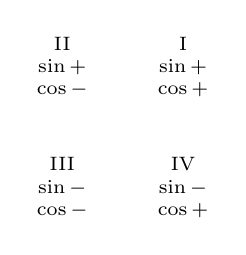
\begin{tikzpicture}[scale=1.75,font=\scriptsize]
  \eenheidscirkel
  \node[align=center] at (45:.62) {I\\$\sin +$\\$\cos +$};
  \node[align=center] at (135:.62) {II\\$\sin +$\\$\cos -$};
  \node[align=center] at (225:.62) {III\\$\sin -$\\$\cos -$};
  \node[align=center] at (315:.62) {IV\\$\sin -$\\$\cos +$};
\end{tikzpicture}}

Omdat de hoeken $\theta$ en $\theta + k \cdot 2\pi$ bij hetzelfde punt horen, hebben ze ook dezelfde coördinaten.

\begin{theorie}
\begin{stelling}{Veelvouden van $2\pi$}
Voor elke hoek $\theta$ en elk geheel getal $k$:

\vspace{1mm}
\qquad $\formule{\sin(\theta + k \cdot 2\pi) = \sin\theta} \qquad \formule{\cos(\theta + k \cdot 2\pi) = \cos\theta}$
\end{stelling}
\begin{bewijs}
De hoek $\theta + k \cdot 2\pi$ is de hoek $\theta$, gevolgd door $k$ volle toeren (in wijzerzin als $k < 0$). Beide hoeken horen dus bij hetzelfde punt $P$, en sinus en cosinus zijn de coördinaten van dat punt.
\end{bewijs}
\end{theorie}

\voorbeeld{}{Bepaal $\sin\frac{7\pi}{2}$, $\cos\frac{7\pi}{2}$ en $\tan\frac{7\pi}{2}$.\label{vb:h1-assen}}{%
\uitleg{De hoek is groter dan $2\pi$. We trekken eerst een volle toer af, zodat we het punt op de cirkel herkennen.}
\begin{stappenbreed}
\tfrac{7\pi}{2} = \tfrac{3\pi}{2} + 2\pi & Een volle toer en nog drie kwart toer. \\
P(0, -1) & Na drie kwart toer sta je onderaan de cirkel. \\
\sin\tfrac{7\pi}{2} = -1, \quad \cos\tfrac{7\pi}{2} = 0 & De coördinaten van $P$. \\
\tan\tfrac{7\pi}{2} \text{ bestaat niet} & De noemer $\cos\frac{7\pi}{2}$ is $0$: de rechte $OP$ staat verticaal.
\end{stappenbreed}}

\begin{oefeningen}
\oef{h1-assen-k}
\end{oefeningen}

\subsection{De grondformule}

In de 2de graad gold $\sin^2\alpha + \cos^2\alpha = 1$ voor een scherpe hoek: dat is de stelling van Pythagoras in de driehoek met schuine zijde $1$. Op de eenheidscirkel geldt dat voor elke hoek. Daarbij betekent $\sin^2\theta$ het kwadraat $(\sin\theta)^2$.

\begin{theorie}
\begin{stelling}{Grondformule}
Voor elke hoek $\theta$: \quad $\formule{\sin^2\theta + \cos^2\theta = 1}$
\end{stelling}
\begin{bewijs}
Het punt $P(\cos\theta, \sin\theta)$ ligt op de eenheidscirkel, dus $|OP| = 1$. Met de afstandsformule is
\bewijsregel{|OP|^2 = (\cos\theta - 0)^2 + (\sin\theta - 0)^2 = 1 ,}
waaruit $\cos^2\theta + \sin^2\theta = 1$.
\end{bewijs}
\end{theorie}

De grondformule zegt dat het punt $(\cos\theta, \sin\theta)$ op de eenheidscirkel ligt. Een gevolg is dat $\sin\theta$ en $\cos\theta$ altijd tussen $-1$ en $1$ liggen. Ken je een van beide, dan ken je de andere op het teken na. Het kwadrant beslist over dat teken.

\voorbeeld{}{Gegeven: $\sin\theta = \frac35$ en $\frac{\pi}{2} < \theta < \pi$. Bepaal $\cos\theta$ en $\tan\theta$.\label{vb:h1-grondformule}}{%
\uitleg{De grondformule geeft $\cos^2\theta$, dus $\cos\theta$ op het teken na. Het kwadrant beslist welk teken het wordt.}
\begin{stappenbreed}
\cos^2\theta = 1 - \sin^2\theta = 1 - \tfrac{9}{25} = \tfrac{16}{25} & Grondformule, opgelost naar $\cos^2\theta$. \\
\cos\theta = \tfrac45 \ \text{ of } \ \cos\theta = -\tfrac45 & Twee getallen hebben dat kwadraat. \\
\cos\theta = -\tfrac45 & $\theta$ ligt in het tweede kwadrant, waar de $x$-coördinaat negatief is. \\[1ex]
\tan\theta = \dfrac{3/5}{-4/5} = -\tfrac34 & De tangens als quotiënt.
\end{stappenbreed}}

\begin{werkwijze}
Bereken het kwadraat van het ontbrekende getal met de grondformule. Bepaal het kwadrant, en kies daarmee het teken van de vierkantswortel. Bereken daarna de tangens als quotiënt.
\end{werkwijze}

\begin{oefeningen}
\oef{h1-grondf}
\end{oefeningen}

Met de grondformule kun je ook uitdrukkingen vereenvoudigen en identiteiten bewijzen: gelijkheden die gelden voor elke hoek waarvoor beide leden bestaan.

\voorbeeld{}{Bewijs: $\dfrac{\cos^2 x}{1 - \sin x} = 1 + \sin x$ (voor $\sin x \neq 1$).\label{vb:h1-identiteit}}{%
\uitleg{In het linkerlid staat $\cos^2 x$, en in de noemer $\sin x$. Met de grondformule schrijven we alles met $\sin x$; dan zien we een merkwaardig product.}
\begin{stappenbreed}
\frac{\cos^2 x}{1 - \sin x} = \frac{1 - \sin^2 x}{1 - \sin x} & Grondformule: $\cos^2 x = 1 - \sin^2 x$. \\[2ex]
= \frac{(1 - \sin x)(1 + \sin x)}{1 - \sin x} & Een verschil van twee kwadraten. \\[2ex]
= 1 + \sin x & Deel door $1 - \sin x$; dat mag, want $\sin x \neq 1$.
\end{stappenbreed}}

\begin{oefeningen}
\oef{h1-ident-k}
\end{oefeningen}

\subsection{Bijzondere waarden}

Voor een paar hoeken ken je sinus en cosinus exact. Je vindt ze altijd terug met de eenheidscirkel en twee driehoeken.

\begin{theorie}
\begin{stelling}{Bijzondere waarden}
\renewcommand{\arraystretch}{1.6}
\begin{tabular}{|c|*{4}{>{\centering\arraybackslash}p{1.25cm}|}>{\centering\arraybackslash}p{2cm}|}
\hline
$\theta$ & $0$ & $\tfrac{\pi}{6}$ & $\tfrac{\pi}{4}$ & $\tfrac{\pi}{3}$ & $\tfrac{\pi}{2}$ \\ \hline
$\sin\theta$ & $\formule{0}$ & $\formule{\tfrac12}$ & $\formule{\tfrac{\sqrt2}{2}}$ & $\formule{\tfrac{\sqrt3}{2}}$ & $\formule{1}$ \\ \hline
$\cos\theta$ & $\formule{1}$ & $\formule{\tfrac{\sqrt3}{2}}$ & $\formule{\tfrac{\sqrt2}{2}}$ & $\formule{\tfrac12}$ & $\formule{0}$ \\ \hline
$\tan\theta$ & $\formule{0}$ & $\formule{\tfrac{\sqrt3}{3}}$ & $\formule{1}$ & $\formule{\sqrt3}$ & bestaat niet \\ \hline
\end{tabular}
\end{stelling}
\begin{bewijs}
\naast{%
Bij $0$ en $\frac{\pi}{2}$ is $P$ het punt $(1, 0)$ en $(0, 1)$.

Bij $\frac{\pi}{4}$ ligt $P$ op de bissectrice $y = x$, dus $x_P = y_P$. Met de grondformule is $2x_P^2 = 1$, en omdat $x_P > 0$:
\bewijsregel{\cos\tfrac{\pi}{4} = \sin\tfrac{\pi}{4} = \tfrac{1}{\sqrt2} = \tfrac{\sqrt2}{2} .}
Bij $\frac{\pi}{3}$ is de driehoek $OAQ$ in de figuur gelijkbenig met tophoek $\frac{\pi}{3}$, dus gelijkzijdig. De hoogte uit $Q$ valt dan in het midden van $[OA]$, zodat $\cos\frac{\pi}{3} = \frac12$.

Bij $\frac{\pi}{6}$ is de driehoek $OPP'$, met $P'$ het spiegelbeeld van $P$ om de $x$-as, gelijkbenig met tophoek $\frac{\pi}{3}$, dus ook gelijkzijdig. Dan is $|PP'| = 2y_P = 1$, zodat $\sin\frac{\pi}{6} = \frac12$.

De andere waarden volgen uit de grondformule (met positieve wortels in het eerste kwadrant), en de tangens als quotiënt.}{%
\begin{tabular}{@{}c@{}}
\begin{tikzpicture}[scale=1.3,font=\scriptsize]
  \eenheidscirkel
  \draw[accent,thick] (0,0) -- (1,0) -- (60:1) -- cycle;
  \draw[accent,dashed] (60:1) -- (.5,0);
  \fill[accent] (60:1) circle (.035) node[above right] {$Q$};
  \node[below left] at (0,0) {$O$};
  \node[below right] at (1,0) {$A$};
  \node[below] at (.5,0) {$\frac12$};
\end{tikzpicture}\\[3mm]
\begin{tikzpicture}[scale=1.3,font=\scriptsize]
  \eenheidscirkel
  \draw[accent,thick] (0,0) -- (30:1) -- (-30:1) -- cycle;
  \fill[accent] (30:1) circle (.035) node[above right] {$P$};
  \fill[accent] (-30:1) circle (.035) node[below right] {$P'$};
  \node[left,accent] at ({cos(30)},.25) {$y_P$};
\end{tikzpicture}
\end{tabular}}
\end{bewijs}
\end{theorie}

\voorbeeld{}{Bereken exact $\sin\frac{\pi}{3}\cos\frac{\pi}{6} - \cos\frac{\pi}{3}\sin\frac{\pi}{6}$.\label{vb:h1-tabel}}{%
\uitleg{Alle hoeken staan in de tabel. We vullen de exacte waarden in en rekenen met breuken en wortels, zonder rekentoestel.}
\begin{stappenbreed}
= \tfrac{\sqrt3}{2} \cdot \tfrac{\sqrt3}{2} - \tfrac12 \cdot \tfrac12 & Waarden uit de tabel. \\
= \tfrac34 - \tfrac14 = \tfrac12 & $\sqrt3 \cdot \sqrt3 = 3$.
\end{stappenbreed}
De uitkomst is $\sin\frac{\pi}{6}$, en $\frac{\pi}{6} = \frac{\pi}{3} - \frac{\pi}{6}$. Dat is geen toeval: in hoofdstuk 2 zie je waarom.}

\needspace{6\baselineskip}
\begin{oefeningen}
\oef{h1-tabel-k}
\end{oefeningen}

%========================================================================================
\section{Verwante hoeken}

Spiegel je het punt $P$ bij $\theta$ om een as of om de oorsprong, dan krijg je punten bij hoeken die met $\theta$ verwant zijn. Hun coördinaten zijn dezelfde, op het teken of de volgorde na. Zo vind je met de tabel van de bijzondere waarden ook sinus en cosinus van hoeken in de andere kwadranten.

\figuren{%
\begin{tikzpicture}[scale=1.25,font=\scriptsize]
  \eenheidscirkel
  \foreach \h/\n/\p in {35/\theta/right,145/\pi - \theta/left,215/\pi + \theta/left,-35/-\theta/right}{
    \draw[accent] (0,0) -- (\h:1);
    \fill[accent] (\h:1) circle (.03) node[\p] {$\n$};}
  \draw[accent,dashed] (35:1) -- (145:1) (35:1) -- (-35:1) (35:1) -- (215:1);
\end{tikzpicture}\hspace{1cm}
\begin{tikzpicture}[scale=1.25,font=\scriptsize]
  \eenheidscirkel
  \draw[grijs,dashed] (-1.1,-1.1) -- (1.2,1.2);
  \foreach \h/\n/\p in {25/\theta/right,65/\frac{\pi}{2} - \theta/above right}{
    \draw[accent] (0,0) -- (\h:1);
    \fill[accent] (\h:1) circle (.03) node[\p] {$\n$};}
\end{tikzpicture}}

In elk bewijs hieronder gebruiken we hetzelfde idee. Een spiegeling om een rechte door $O$ brengt de eenheidscirkel over in zichzelf, maar keert de draaizin om: tegenwijzerzin wordt wijzerzin.

\subsection{Tegengestelde hoeken}

De hoeken $\theta$ en $-\theta$ draaien even ver, maar in tegengestelde zin. Hun punten zijn elkaars spiegelbeeld om de $x$-as.

\begin{theorie}
\begin{stelling}{Tegengestelde hoeken}
\qquad $\formule{\sin(-\theta) = -\sin\theta} \qquad \formule{\cos(-\theta) = \cos\theta} \qquad \formule{\tan(-\theta) = -\tan\theta}$
\end{stelling}
\begin{bewijs}
Spiegel om de $x$-as. Het vertrekpunt $(1, 0)$ blijft liggen en de draaizin keert om, dus het punt $P$ bij $\theta$ gaat naar het punt bij $-\theta$. Die spiegeling behoudt $x$ en verandert het teken van $y$:
\bewijsregel{\bigl(\cos(-\theta), \sin(-\theta)\bigr) = (\cos\theta, -\sin\theta) .}
Delen geeft $\tan(-\theta) = \dfrac{-\sin\theta}{\cos\theta} = -\tan\theta$.
\end{bewijs}
\end{theorie}

De cosinus merkt dus niets van het teken van de hoek; sinus en tangens wisselen van teken.

\voorbeeld{}{Bepaal exact $\tan\bigl(-\frac{\pi}{3}\bigr)$.\label{vb:h1-tegengesteld}}{%
\uitleg{De hoek $-\frac{\pi}{3}$ is het tegengestelde van een hoek uit de tabel. Het punt ligt in het vierde kwadrant.}
\begin{stappenbreed}
\tan\bigl(-\tfrac{\pi}{3}\bigr) = -\tan\tfrac{\pi}{3} & Tegengestelde hoeken. \\
= -\sqrt3 & Bijzondere waarde.
\end{stappenbreed}
Controle met het kwadrant: in het vierde kwadrant is $\sin\theta < 0$ en $\cos\theta > 0$, dus de tangens is negatief.}

\begin{oefeningen}
\oef{h1-tegen-k}
\end{oefeningen}

\subsection{Supplementaire hoeken}

Twee hoeken zijn supplementair als hun som $\pi$ is, zoals $\theta$ en $\pi - \theta$. Hun punten zijn elkaars spiegelbeeld om de $y$-as.

\begin{theorie}
\begin{stelling}{Supplementaire hoeken}
\qquad $\formule{\sin(\pi - \theta) = \sin\theta} \qquad \formule{\cos(\pi - \theta) = -\cos\theta} \qquad \formule{\tan(\pi - \theta) = -\tan\theta}$
\end{stelling}
\begin{bewijs}
Spiegel om de $y$-as. Het vertrekpunt $(1, 0)$ gaat naar $(-1, 0)$, het punt bij $\pi$, en de draaizin keert om. Een draaiing over $\theta$ vanaf $(1, 0)$ wordt dus een draaiing over $\theta$ in wijzerzin vanaf het punt bij $\pi$: het beeld van $P$ hoort bij $\pi - \theta$. Die spiegeling verandert het teken van $x$ en behoudt $y$:
\bewijsregel{\bigl(\cos(\pi - \theta), \sin(\pi - \theta)\bigr) = (-\cos\theta, \sin\theta) .}
Delen geeft $\tan(\pi - \theta) = \dfrac{\sin\theta}{-\cos\theta} = -\tan\theta$.
\end{bewijs}
\end{theorie}

Supplementaire hoeken hebben dus dezelfde sinus. Daarom heeft een vergelijking als $\sin x = \frac12$ twee oplossingen in $[0, 2\pi[$: dat zie je in hoofdstuk 4.

\voorbeeld{}{Bepaal exact $\sin\frac{5\pi}{6}$, $\cos\frac{5\pi}{6}$ en $\tan\frac{5\pi}{6}$.\label{vb:h1-waarden}}{%
\naast{%
\uitleg{$\frac{5\pi}{6} = \pi - \frac{\pi}{6}$: een supplementaire hoek van $\frac{\pi}{6}$. Het punt is het spiegelbeeld van het punt bij $\frac{\pi}{6}$ om de $y$-as: dezelfde hoogte, tegengestelde $x$.}
\begin{stappenvrij}{4cm}{3.6cm}
\sin\tfrac{5\pi}{6} = \sin\tfrac{\pi}{6} = \tfrac12 & Zelfde $y$. \\
\cos\tfrac{5\pi}{6} = -\cos\tfrac{\pi}{6} = -\tfrac{\sqrt3}{2} & Tegengestelde $x$. \\
\tan\tfrac{5\pi}{6} = -\tfrac{1}{\sqrt3} = -\tfrac{\sqrt3}{3} & $\sin$ gedeeld door $\cos$.
\end{stappenvrij}}{%
\begin{tikzpicture}[scale=1.4,font=\scriptsize]
  \eenheidscirkel
  \draw[accent] (0,0) -- (30:1) (0,0) -- (150:1);
  \draw[accent,dashed] (30:1) -- (150:1);
  \fill[accent] (30:1) circle (.03) node[right] {$\frac{\pi}{6}$};
  \fill[accent] (150:1) circle (.03) node[left] {$\frac{5\pi}{6}$};
\end{tikzpicture}}}

\begin{oefeningen}
\oef{h1-waarden}
\end{oefeningen}

\subsection{Antisupplementaire hoeken}

De hoeken $\theta$ en $\pi + \theta$ verschillen een halve toer. Hun punten liggen diametraal tegenover elkaar: ze zijn elkaars spiegelbeeld om de oorsprong. Het bewijs volgt nu uit de twee vorige eigenschappen.

\begin{theorie}
\begin{stelling}{Antisupplementaire hoeken}
\qquad $\formule{\sin(\pi + \theta) = -\sin\theta} \qquad \formule{\cos(\pi + \theta) = -\cos\theta} \qquad \formule{\tan(\pi + \theta) = \tan\theta}$
\end{stelling}
\begin{bewijs}
Schrijf $\pi + \theta = \pi - (-\theta)$. Gebruik eerst supplementaire en daarna tegengestelde hoeken:
\bewijsregel{\sin(\pi + \theta) = \sin\bigl(\pi - (-\theta)\bigr) = \sin(-\theta) = -\sin\theta}
\bewijsregel{\cos(\pi + \theta) = \cos\bigl(\pi - (-\theta)\bigr) = -\cos(-\theta) = -\cos\theta}
Delen geeft $\tan(\pi + \theta) = \dfrac{-\sin\theta}{-\cos\theta} = \tan\theta$.
\end{bewijs}
\end{theorie}

Een halve toer verder keren beide coördinaten van teken, en hun quotiënt blijft gelijk. De tangens herhaalt zich dus al na $\pi$, en niet pas na $2\pi$.

\voorbeeld{}{Bepaal exact $\cos\frac{4\pi}{3}$.\label{vb:h1-verwant}}{%
\uitleg{$\frac{4\pi}{3} = \pi + \frac{\pi}{3}$: een antisupplementaire hoek van $\frac{\pi}{3}$. Het punt ligt in het derde kwadrant.}
\begin{stappenbreed}
\cos\tfrac{4\pi}{3} = \cos\bigl(\pi + \tfrac{\pi}{3}\bigr) = -\cos\tfrac{\pi}{3} & Antisupplementair. \\
= -\tfrac12 & Bijzondere waarde. In het derde kwadrant is de cosinus inderdaad negatief.
\end{stappenbreed}}

\begin{oefeningen}
\oef{h1-punt}
\end{oefeningen}

\subsection{Complementaire hoeken}

Twee hoeken zijn complementair als hun som $\frac{\pi}{2}$ is, zoals $\theta$ en $\frac{\pi}{2} - \theta$. Hun punten zijn elkaars spiegelbeeld om de rechte $y = x$.

\begin{theorie}
\begin{stelling}{Complementaire hoeken}
\qquad $\formule{\sin\bigl(\tfrac{\pi}{2} - \theta\bigr) = \cos\theta} \qquad \formule{\cos\bigl(\tfrac{\pi}{2} - \theta\bigr) = \sin\theta} \qquad \formule{\tan\bigl(\tfrac{\pi}{2} - \theta\bigr) = \frac{1}{\tan\theta}}$

\vspace{1mm}
de laatste voor $\theta \neq k \cdot \frac{\pi}{2}$ ($k \in \Z$).
\end{stelling}
\begin{bewijs}
Spiegel om de rechte $y = x$. Het vertrekpunt $(1, 0)$ gaat naar $(0, 1)$, het punt bij $\frac{\pi}{2}$, en de draaizin keert om. Het beeld van $P$ hoort dus bij $\frac{\pi}{2} - \theta$. Die spiegeling wisselt de coördinaten:
\bewijsregel{\bigl(\cos(\tfrac{\pi}{2} - \theta), \sin(\tfrac{\pi}{2} - \theta)\bigr) = (\sin\theta, \cos\theta) .}
Delen geeft $\tan\bigl(\frac{\pi}{2} - \theta\bigr) = \dfrac{\cos\theta}{\sin\theta} = \dfrac{1}{\tan\theta}$, als $\sin\theta \neq 0$ en $\cos\theta \neq 0$.
\end{bewijs}
\end{theorie}

Hier komt de naam \textit{cosinus} vandaan: het is de sinus van de complementaire hoek. In een rechthoekige driehoek zijn de twee scherpe hoeken complementair, en de overstaande zijde van de ene is de aanliggende zijde van de andere.

\voorbeeld{}{Vereenvoudig $\sin\bigl(\frac{\pi}{2} - x\bigr)\cos x + \cos\bigl(\frac{\pi}{2} - x\bigr)\sin x$.\label{vb:h1-compl}}{%
\uitleg{Twee hoeken zijn van de vorm $\frac{\pi}{2} - x$. Met complementaire hoeken schrijven we alles met de hoek $x$.}
\begin{stappenbreed}
= \cos x \cdot \cos x + \sin x \cdot \sin x & Complementaire hoeken. \\
= \cos^2 x + \sin^2 x = 1 & Grondformule.
\end{stappenbreed}}

\begin{oefeningen}
\oef{h1-compl-k}
\end{oefeningen}

\needspace{16\baselineskip}
\subsection{Een hoek herleiden}

Met de veelvouden van $2\pi$ en de vier soorten verwante hoeken herleid je sinus, cosinus en tangens van elke hoek tot die van een hoek tussen $0$ en $\frac{\pi}{2}$.

\voorbeeld{}{Bepaal exact $\cos\frac{23\pi}{4}$.\label{vb:h1-herleiden}}{%
\uitleg{De hoek is bijna drie volle toeren. We trekken die toeren af, en herkennen dan een verwante hoek van $\frac{\pi}{4}$.}
\begin{stappenbreed}
\tfrac{23\pi}{4} - 3 \cdot 2\pi = \tfrac{23\pi}{4} - \tfrac{24\pi}{4} = -\tfrac{\pi}{4} & Drie toeren eraf: dezelfde cosinus. \\
\cos\tfrac{23\pi}{4} = \cos\bigl(-\tfrac{\pi}{4}\bigr) = \cos\tfrac{\pi}{4} & Tegengestelde hoeken. \\
= \tfrac{\sqrt2}{2} & Het punt ligt in het vierde kwadrant: de cosinus is positief.
\end{stappenbreed}}

\begin{werkwijze}
Trek veelvouden van $2\pi$ af tot de hoek tussen $-\pi$ en $\pi$ (of tussen $0$ en $2\pi$) ligt. Schrijf hem als $\pi - \alpha$, $\pi + \alpha$ of $-\alpha$ met $\alpha$ tussen $0$ en $\frac{\pi}{2}$. Gebruik de verwante hoeken, en controleer het teken met het kwadrant.
\end{werkwijze}

\nujij{Bepaal exact $\sin\bigl(-\frac{7\pi}{4}\bigr)$.}{$-\frac{7\pi}{4} + 2\pi = \frac{\pi}{4}$, dus $\sin\bigl(-\frac{7\pi}{4}\bigr) = \sin\frac{\pi}{4} = \frac{\sqrt2}{2}$.}

\begin{oefeningen}
\oef{h1-verwant}

\oef{h1-herleid}
\end{oefeningen}

%========================================================================================
\opdrachtenkop

\begin{oefeningen}
\needspace{10\baselineskip}
\oef{h1-o1}

\needspace{12\baselineskip}
\oef{h1-o10}

\oef{h1-o13}

\needspace{10\baselineskip}
\oef{h1-o2}

\needspace{12\baselineskip}
\oef{h1-o11}

\needspace{12\baselineskip}
\oef{h1-o14}

\oef{h1-o3}

\oef{h1-o15}

\oef{h1-o12}

\oef{h1-o4}

\oef{h1-o16}

\oef{h1-o5}

\needspace{12\baselineskip}
\oef{h1-o17}

\oef{h1-o7}

\needspace{10\baselineskip}
\oef{h1-o20}

\oef{h1-o6}

\oef{h1-o22}

\oef{h1-o19}

\needspace{14\baselineskip}
\oef{h1-o18}

\oef{h1-o23}

\needspace{12\baselineskip}
\oef{h1-o21}

\needspace{14\baselineskip}
\oef{h1-o24}

\oef{h1-o8}

\oef{h1-o26}

\needspace{16\baselineskip}
\oef{h1-o25}

\oef{h1-o9}
\end{oefeningen}

%----------------------------------------------------------------------------------------
% KOPPEL: verbanden met andere leerstof
%----------------------------------------------------------------------------------------
\needspace{20\baselineskip}
\opdrachtsectie{Koppel}

\lkr{Algemene functies en Matrices: kijk na wat al gezien is. Het pakket legt de volgorde niet vast.}

\begin{oefeningen}

\oef{h1-koppel-2}

\oef{h1-koppel-3}
\end{oefeningen}

%----------------------------------------------------------------------------------------
\opdrachtsectie{Test jezelf}

\begin{oefeningen}
\oef{h1-t1}

\oef{h1-t2}

\oef{h1-t3}

\oef{h1-t4}

\oef{h1-t5}

\oef{h1-t6}

\oef{h1-t7}

\oef{h1-t8}
\end{oefeningen}

\herhaalschema{%
  \fv{oef:h1-t1}{vb:h1-radialen}{oef:h1-radialen}%
  \fv{oef:h1-t2}{vb:h1-sector}{oef:h1-sector}%
  \fv{oef:h1-t3}{vb:h1-waarden}{oef:h1-waarden}%
  \fv{oef:h1-t4}{vb:h1-grondformule}{oef:h1-grondf}%
  \fv{oef:h1-t5}{vb:h1-herleiden}{oef:h1-herleid}%
  \fv{oef:h1-t6}{vb:h1-verwant}{oef:h1-punt}%
  \fv{oef:h1-t7}{vb:h1-compl}{oef:h1-verwant}%
  \fv{oef:h1-t8}{vb:h1-identiteit}{oef:h1-ident-k}}

\ifzelfstudie
\section*{Maak je eigen samenvatting}
Sluit dit boek en schrijf in je schrift: de definitie van een radiaal, het omrekenen, booglengte en sectoroppervlakte, de definities van $\sin$, $\cos$ en $\tan$ op de eenheidscirkel, de grondformule, de tabel met bijzondere waarden en de vier soorten verwante hoeken, telkens met een figuur. Vergelijk daarna met de kaders.
\fi
